\documentclass[tikz,border=5pt]{standalone}
\usetikzlibrary{calc, arrows.meta}

\begin{document}

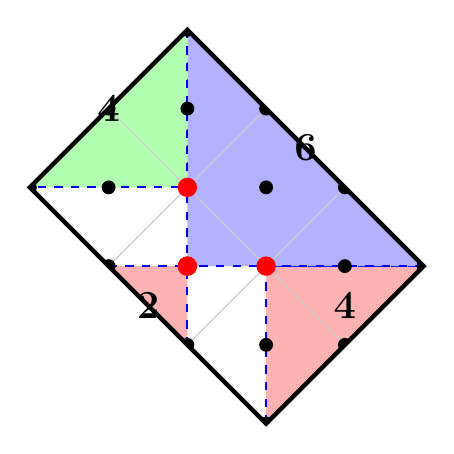
\begin{tikzpicture}[scale=1]
    % 1. Vertices of the rectangle
    \coordinate (A) at (0,0);
    \coordinate (B) at (3,-3);
    \coordinate (C) at (5,-1);
    \coordinate (D) at (2,2);

    % 2. Surgery Apexes
    \coordinate (P1) at (2,-1); % T1 apex (Red)
    \coordinate (P2) at (3,-1); % T2 apex (Red)
    \coordinate (P3) at (2,-1); % T3 apex (Blue)
    \coordinate (P4) at (2,0);  % T4 apex (Green)

    % 3. Surgery Shading (Symington surgeries)
    % T1: Red, Basis Triangle (1,-1)-(2,-2) to (2,-1)
    \fill[red!30] (1,-1) -- (2,-2) -- (P1) -- cycle;
    \draw[blue, thick, dashed] (1,-1) -- (P1) -- (2,-2);
    
    % T2: Red, Apex (3,-1), base is entire Edge 2 (BC)
    \fill[red!30] (B) -- (C) -- (P2) -- cycle;
    \draw[blue, thick, dashed] (B) -- (P2) -- (C);
    
    % T3: Blue, Apex (2,-1), base is entire Edge 3 (CD)
    \fill[blue!30] (C) -- (D) -- (P3) -- cycle;
    \draw[blue, thick, dashed] (C) -- (P3) -- (D);
    
    % T4: Green, Apex (2,0), base is entire Edge 4 (DA)
    \fill[green!30] (D) -- (A) -- (P4) -- cycle;
    \draw[blue, thick, dashed] (D) -- (P4) -- (A);

    % 4. Lattice Triangulation
    \begin{scope}[gray!40, thin]
        \clip (A) -- (B) -- (C) -- (D) -- cycle;
        \foreach \k in {-10,...,10} {
            \draw (\k-10, -\k-10) -- (\k+10, -\k+10);
            \draw (\k-10, \k+10) -- (\k+10, \k-10);
        }
    \end{scope}

    % 5. Polytope Boundary
    \draw[ultra thick, black] (A) -- (B) -- (C) -- (D) -- cycle;

    % 6. Lattice Nodes (Z2)
    \begin{scope}
        \clip (A) -- (B) -- (C) -- (D) -- cycle;
        \foreach \x in {0,...,6} {
            \foreach \y in {-4,...,2} {
                \fill (\x, \y) circle (2.5pt);
            }
        }
    \end{scope}

    % Highlight surgery apexes
    \foreach \p in {P1, P2, P3, P4} {
        \fill[red] (\p) circle (3.5pt);
    }

    % 7. Labels
    \node[font=\Large\bfseries] at (1.5, -1.5) {2};
    \node[font=\Large\bfseries] at (4, -1.5) {4};
    \node[font=\Large\bfseries] at (3.5, 0.5) {6};
    \node[font=\Large\bfseries] at (1, 1) {4};

\end{tikzpicture}

\end{document}
